%% Преамбула TeX-файла

% 1. Стиль и язык
\documentclass[pscyr, 12pt]{G7-32} % Стиль (по умолчанию размер шрифта 14pt)

% Остальные стандартные настройки убраны в preamble.inc.tex.
\sloppy

% Настройки стиля ГОСТ 7-32
% Для начала определяем, хотим мы или нет, чтобы рисунки и таблицы нумеровались в пределах раздела, или нам нужна сквозная нумерация.
\EqInChapter % формулы будут нумероваться в пределах раздела
\TableInChapter % таблицы будут нумероваться в пределах раздела
\PicInChapter % рисунки будут нумероваться в пределах раздела

% Добавляем гипертекстовое оглавление в PDF
\usepackage[
bookmarks=true, colorlinks=true, unicode=true,
urlcolor=black,linkcolor=black, anchorcolor=black,
citecolor=black, menucolor=black, filecolor=black,
]{hyperref}

\AfterHyperrefFix

\usepackage{microtype}% полезный пакет для микротипографии, увы под xelatex мало чего умеет, но под pdflatex хорошо улучшает читаемость

% Тире могут быть невидимы в Adobe Reader
\ifInvisibleDashes
\MakeDashesBold
\fi

\usepackage{graphicx}   % Пакет для включения рисунков

% С такими оно полями оно работает по-умолчанию:
% \RequirePackage[left=20mm,right=10mm,top=20mm,bottom=20mm,headsep=0pt,includefoot]{geometry}
% Если вас тошнит от поля в 10мм --- увеличивайте до 20-ти, ну и про переплёт не забывайте:
\geometry{right=10mm}
\geometry{left=30mm}
\geometry{bottom=20mm}
\geometry{ignorefoot}% считать от нижней границы текста


% Пакет Tikz
\usepackage{tikz}
\usetikzlibrary{arrows,positioning,shadows}

% Произвольная нумерация списков.
\usepackage{enumerate}

% ячейки в несколько строчек
\usepackage{multirow}

% itemize внутри tabular
\usepackage{paralist,array}

%\setlength{\parskip}{1ex plus0.5ex minus0.5ex} % разрыв между абзацами
\setlength{\parskip}{1ex} % разрыв между абзацами
\usepackage{blindtext}

% Центрирование подписей к плавающим окружениям
%\usepackage[justification=centering]{caption}

\usepackage{newfloat}
\DeclareFloatingEnvironment[
placement={!ht},
name=Equation
]{eqndescNoIndent}
\edef\fixEqndesc{\noexpand\setlength{\noexpand\parindent}{\the\parindent}\noexpand\setlength{\noexpand\parskip}{\the\parskip}}
\newenvironment{eqndesc}[1][!ht]{%
    \begin{eqndescNoIndent}[#1]%
\fixEqndesc%
}
{\end{eqndescNoIndent}}


% Настройки листингов.
\ifPDFTeX
% 8 Листинги

\usepackage{listings}

% Значения по умолчанию
\lstset{
  numberbychapter=false,
  basicstyle= \small\ttfamily,
  breakatwhitespace=true,% разрыв строк только на whitespacce
  breaklines=true,       % переносить длинные строки
%   captionpos=b,          % подписи снизу -- вроде не надо
  inputencoding=utf8,
  basewidth=0.5em,
  extendedchars=\true,
  numberstyle=\footnotesize,
  showspaces=false,      % показывать пробелы подчеркиваниями -- идиотизм 70-х годов
  showstringspaces=false,
  showtabs=false,        % и табы тоже
  stepnumber=1,
  numbers=left,
  numbersep=10pt,
  tabsize=4,              % кому нужны табы по 8 символов?
  frame=lines,
  lineskip=0.1em,
  keepspaces=true,
  framexleftmargin=1.5em,
  xleftmargin=1.5em
}

% Стиль для псевдокода: строчки обычно короткие, поэтому размер шрифта побольше
\lstdefinestyle{pseudocode}{
  basicstyle=\small,
  keywordstyle=\color{black}\bfseries\underbar,
  language=Pseudocode,
  numberstyle=\footnotesize,
  commentstyle=\footnotesize\it
}

% Стиль для обычного кода: маленький шрифт
\lstdefinestyle{realcode}{
  basicstyle=\scriptsize,
  numberstyle=\footnotesize
}

% Стиль для коротких кусков обычного кода: средний шрифт
\lstdefinestyle{simplecode}{
  basicstyle=\footnotesize,
  numberstyle=\footnotesize
}

% Стиль для BNF
\lstdefinestyle{grammar}{
  basicstyle=\footnotesize,
  numberstyle=\footnotesize,
  stringstyle=\bfseries\ttfamily,
  language=BNF
}

% Определим свой язык для написания псевдокодов на основе Python
\lstdefinelanguage[]{Pseudocode}[]{Python}{
  morekeywords={each,empty,wait,do},% ключевые слова добавлять сюда
  morecomment=[s]{\{}{\}},% комменты {а-ля Pascal} смотрятся нагляднее
  literate=% а сюда добавлять операторы, которые хотите отображать как мат. символы
    {->}{\ensuremath{$\rightarrow$}~}2%
    {<-}{\ensuremath{$\leftarrow$}~}2%
    {:=}{\ensuremath{$\leftarrow$}~}2%
    {<--}{\ensuremath{$\Longleftarrow$}~}2%
}[keywords,comments]

% Свой язык для задания грамматик в BNF
\lstdefinelanguage[]{BNF}[]{}{
  morekeywords={},
  morecomment=[s]{@}{@},
  morestring=[b]",%
  literate=%
    {->}{\ensuremath{$\rightarrow$}~}2%
    {*}{\ensuremath{$^*$}~}2%
    {+}{\ensuremath{$^+$}~}2%
    {|}{\ensuremath{$|$}~}2%
}[keywords,comments,strings]

\lstdefinelanguage{Nix}{
  % Anything betweeen $ becomes LaTeX math mode
  mathescape=false,
  % Comments may or not include Latex commands
  texcl=false,
  keywords=[1]{inherit,import,if,then,else,false,true,or,rec,let,in,assert,with},
  % Comments delimiters, we do turn this off for the manual
  % Spaces are not displayed as a special character
  showstringspaces=false,
  % String delimiters
  morestring=[b]",
  morestring=[d]'',
  % Size of tabulations
  tabsize=2,
  % Enables ASCII chars 128 to 255
  sensitive=true,
  columns=[l]fixed,
}

% Подписи к листингам на русском языке.
\renewcommand\lstlistingname{Листинг}
\renewcommand\lstlistlistingname{Листинги}

\else
\usepackage{local-minted}
\fi

% Полезные макросы листингов.
% Любимые команды
\newcommand{\Code}[1]{\textbf{#1}}


% Стиль титульного листа и заголовки
%\NirEkz{Экз. 3}                                  % Раскоментировать если не требуется
%\NirGrif{Секретно}                % Наименование грифа

\gosttitle{Gost7-32}       % Шаблон титульной страницы, по умолчанию будет ГОСТ 7.32-2001,
% Варианты GostRV15-110 или Gost7-32

\NirOrgLongName{МИНИСТЕРСТВО НАУКИ И ВЫСШЕГО ОБРАЗОВАНИЯ \\
РОССИЙСКОЙ ФЕДЕРАЦИИ\\[1em]
Федеральное государственное автономное учреждение высшего образования\\
<<МОСКОВСКИЙ ПОЛИТЕХНИЧЕСКИЙ УНИВЕРСИТЕТ>>
}                                           %% Полное название организации

\NirUdk{ }
\NirGosNo{ }
\NirInventarNo{ }

\NirConfirm{Допущен к защите}                  % Смена УТВЕРЖДАЮ
\NirBoss[.49]{Руководитель образовательной программы <<Безопасность компьютерных систем>>}{/ А. Ю. Гневшев /}            %% Заказчик, утверждающий НИР

\NirReportName{Выпускная квалификационная работа}   % Можно поменять тип отчета
\NirAbout{} %Можно изменить о чем отчет

%\NirPartNum{Часть}{1}                      % Часть номер

\NirBareSubject{}                  % Убирает по теме если раскоментить

\Nir{по направлению \par
        10.03.01 Информационная безопасность \par
        (бакалавр) \par
        Образовательная программа (профиль) \par
        <<Безопасность компьютерных систем>> \par
        на тему:}

\NirSubject{<<Проектирование и разработка среды для проведения дистанционных испытаний в области защиты информации>>}                                   % Наименование темы
\NirFinal{}                        % Заключительный, если закоментировать то промежуточный
\finalname{черновая}               %п Название финального отчета (Заключительный)
%\NirCode{Шифр\,---\,САПР-РЛС-ФИЗТЕХ-1} % Можно задать шифр как в ГОСТ 15.110
\NirCode{}

\NirManager{Руководитель ВКР}{А. С. Красников, к.ф-м.н.} %% Название руководителя
\NirIsp{Студент}{И. С. Клименко, гр. 181-351} %% Название руководителя

\NirYear{2022}%% если нужно поменять год отчёта; если закомментировано, ставится текущий год
\NirTown{Москва ---}                           %% город, в котором написан отчёт



\begin{document}


\frontmatter % выключает нумерацию ВСЕГО; здесь начинаются ненумерованные главы: реферат, введение, глоссарий, сокращения и прочее.

\maketitle %создает титульную страницу


%% \begin{executors}
%% \personalSignature{Первый исполнитель}{ФИО}

%% \personalSignature{Второй исполнитель}{ФИО}
%% \end{executors}


%\listoffigures                         % Список рисунков

%\listoftables                          % Список таблиц

%\NormRefs % Нормативные ссылки
% Команды \breakingbeforechapters и \nonbreakingbeforechapters
% управляют разрывом страницы перед главами.
% По-умолчанию страница разрывается.

% \nobreakingbeforechapters
% \breakingbeforechapters

% Также можно использовать \Referat, как в оригинале

\pagestyle{empty}

\chapter*{Аннотация}

Наименование работы: <<Программная среда для проведения дистанционных испытаний в области защиты информации>>.

Цель работы: спроектировать и разработать среду для проведения дистанционных испытаний в области защиты информации.

Объект исследования работы --- программно-аппаратная среда для проведения всероссийской школьной олимпиады по защите информации Ugra CTF School.

Работа состоит из введения, трёх глав, заключения и приложений. Общий объём работы --- \pageref{LastPage}, из них 2 приложения на 63 листах. В работу включены 14 рисунков, 6 таблиц. Библиографический список состоит из 75 источников: 37 электронных ресурсов и 38 печатных текстов.

Введение содержит обоснование актуальности выбранной темы, цель и задачи аттестационной работы.

Первая глава содержит историческую справку о соревнованиях в области защиты информации, правила и принципы их проведения, сведения об олимпиаде Ugra CTF и её организационных особенностях. В этой главе вводится понятие CTF-соревнований и распределённо-очного формата проведения школьных олимпиад.

Вторая глава посвящена изучению организационных, технических и правовых требований, предъявляемых к проведению олимпиады Ugra CTF и теоретическим изысканиям, которые связаны с проектированием среды для проведения этой олимпиады.

В третьей главе изложены сведения об итоговой архитектуре автоматизированной системы, обеспечивающей создание и управление средой для проведения испытаний, а также технические детали её реализации.

В заключении формулируются выводы о проделанной работе и описывается ход апробации разработанной системы на практике, в реальных условиях олимпиады Ugra CTF School 2022, которая прошла 2 апреля 2022 года одновременно в 10 городах России.

\pagestyle{empty}
\chapter*{Abstract}

Title: ``Software environment for conducting remote information security challenges''.

The object of the research is a computer environment for all-Russian school Olympiad on information security, Ugra CTF School.

The work consists of an introduction, three chapters, a conclusion and appendices. This work spans \pageref{LastPage} pages, 63 of which are the 2 appendices. The paper comprises 14 figures, 6 tables. Bibliography list comprises 75 sources: 37 electronic resources and 38 printed texts.

In the introduction we express the rationale for picking this topic, and state the purpose and objectives of this work.

In the first chapter we review the historical background of the information security competitions, their rules, and organizational nuances of Ugra CTF Olympiad. This chapter introduces the notion of a CTF competition and the distributed format of the school Olympiads.

In the second chapter we study organizational, technical and legal requirements for conducting the Ugra CTF --- and explore theoretical questions involved with the design of an automated system for providing a computer environment for participants to solve Olympiad's challenges.

In the third chapter we review the final architecture of the system, as well as the details of its implementation.

In the conclusion we analyze the results and describe the progress of testing the developed system at a real event, during the Ugra CTF School 2022 Olympiad, which was held on April 2, 2022 simultaneously in 10 cities of Russia.

%%% Local Variables:
%%% mode: latex
%%% TeX-master: "rpz"
%%% End:


\tableofcontents

\printnomenclature % Автоматический список сокращений

\Introduction
Безопасность информации — актуальный вопрос, поскольку по мере роста значимости киберпространства и развития технологий, растёт и серьёзность угроз, которые в нём возникают. При текущих треднах будущим поколениям придётся столкнуться с куда более серьёзными вызовами и сложностями в этой сфере, о которых сегодня можно лишь догадываться: например, в последнее время более активно, чем прежде, проводятся исследования в области квантовых вычислений\cite{Quantum1}\cite{Quantum2}, успех в которых гарантированно приведёт к утрате стойкости всех распространённых криптографических методов\cite{Quantum3}.

Один из способов повышения осведомлённости о проблемах кибербезопасности — внедрение её азов в формате школьных олимпиад.

С 2016 года в России проводится школьная олимпиада по защите информации Ugra CTF\cite{UgraHistory}. За её организацию отвечает Югорский научно-исследовательский институт информационных технологий, практику в котором проходит автор настоящей работы.

Проведение мероприятий подобного уровня, с одной стороны, требует полного соблюдения требований Российского совета олимпиад школьников\cite{Rosolymp}, которые в строгом порядке регламентируют действия как участников, так и организаторов. С другой стороны, для этого необходимо создать участникам максимально приближенные к настоящим условия для демонстрации своих навыков в сфере практической кибербезопасности — по этой причине они проводятся в формате CTF \textit{(англ. capture the flag, «захват флага»)}. Формат игровой: участники исследуют модели компьютерных систем на предмет уязвимостей, эксплуатация либо устранение которых приносит очки.

Основная сложность заключается в том, что заключительный этап олимпиады --- очный и проводится более чем в десяти городах по всей стране\cite{Statforma}. Организационно-технический процесс, включающий в себя подготовку рабочих мест участников, настройку инфраструктуры и дистанционный контроль за ходом мероприятия на разных площадках, можно сделать эффективнее, разработав и внедрив в него элементы автоматизации.

Цель данной выпускной квалификационной работы --- спроектировать и разработать среду для проведения дистанционных испытаний в области защиты информации.

Проектирование и разработка такой среды достигается решением следующих задач:
\begin{itemize}
\item изучить особенности проведения испытаний в формате: требования РСОШ, принципы и правила CTF-соревнований;
\item разработать перечень технических требований к среде для проведения дистанционных испытаний;
\item спроектировать архитектуру среды и описать принципы её работы;
\item создать автоматизированную систему (АС) для управления такой средой.
\Abbrev{АС}{автоматизированная система}
\end{itemize}


\mainmatter % это включает нумерацию глав и секций в документе ниже

\chapter{Аналитическая часть: введение в понятие соревнований по защите информации}
\label{cha:analysis}

\section{История}

Согласно «Словарю русского языка» C. И. Ожегова, соревнования --- форма деятельности (работы, игры), при которой участвующие стремятся превзойти друг друга \cite{Ozhegov89}. По моему мнению, вышеупомянутое стремление есть неотъемлемая часть человеческой природы и один из определяющих факторов развития нашей цивилизации, ведь прогресс в любой сфере деятельности --- это достижение новых, более совершенных результатов в чём бы то ни было.

\Abbrev{ICPC}{International Collegiate Programming Contest ""--- Международная студенческая олимпиада по программированию}

Соревнования естественным образом возникают и в областях, связанных с информационными технологиями. Так, в 1970 году в Техасском университете A\&M были проведены соревнования по спортивному программированию, ныне известные как ICPC\cite{AboutICPC}. Командам участников предлагали решить несколько формально определённых задач на языке программирования «Фортран». Организаторы засекали время и принимали решения на перфокартах: призовые места распределялись согласно времени, которое команда потратила на решение.

На сегодняшний день ICPC — масштабное, уважаемое и значимое соревнование, к победе в котором стремятся сотни тысяч студентов технических вузов по всему миру. Возникли и другие соревнования по спортивному программированию, например, Всероссийская олимпиада школьников по информатике.

Когорта спортивных программистов внесла существенный вклад в развитие науки и техники. Опыт, получаемый во время тренировок и непосредственного участия в соревнованиях, отразился в компьютерных науках (теория алгоритмов, теория оптимизации, численные методы и др.), методиках преподавания связанных с разработкой программного обеспечения дисциплин и проч. В качестве примера можно привести открытую в 2000 году многократным победителем олимпиад по программированию Николаем Дуровым структуру данных, известную как \textit{декартово дерево по неявному ключу}\cite{Durov00} или возникновение в России системы компьютерных школ и сборов, воспитавших не одно поколение талантливых программистов, архитекторов и учёных\cite{Netrusova09}\cite{Kraivanova12}.

По мере распространения компьютерных технологий закономерно всё актуальнее становился вопрос о их безопасности. Возникло понятние кибербезопасности --- совокупности методов и практик защиты от атак злоумышленников для компьютеров, серверов, мобильных устройств, электронных систем, сетей и данных. И в этой сфере появились свои соревнования. Они проходят в формате CTF \textit{(англ. capture the flag --- «захват флага»)}.

\Define{Кибербезопасность}{совокупность методов и практик защиты от атак злоумышленников для компьютеров, серверов, мобильных устройств, электронных систем, сетей и данных}

\Abbrev{CTF}{capture the flag ""--- формат соревнований по защите информации «захват флага»}

Первые в мире соревнования по защите в таком формате, DEF CON CTF, были проведены в США в 1996 году \cite{Defcon}. Они проходили следующим образом. Организаторы предоставили командам участников модельную компьютерную систему --- некий программный сервис, который принимает пользовательские запросы и неким соответствующим образом их обратывающий. В базе данных сервиса хранились т.н. флаги --- текстовые строки определённого формата, на месте которых в реальной, не модельной, ситуации могли бы оказаться критически важные данные: например, номера банковских карт или пароли. Наконец, в системе были предусмотрены определённые уявзимости, с помощью которых. От участников требовалось запустить предоставленный сервис на своём сервере, доступном из общей игровой сети, поддерживать его в работоспособном состоянии, обнаруживая и исправляя в нём уязвимости; а также использовать найденные уязвимости для «захвата» флагов с аналогичных серверов других команд.

Со временем CTF-соревнования стали массовым явлением. Свои мероприятия проводят такие крупные IT-комании, как Meta\cite{FBCTF}, Google\cite{GoogleCTF}, «Яндекс»\cite{YaCTF} и «Лаборатория Касперского»\cite{KasperskyCTF}. За участие в них победителям выплачивают крупные денежные призы, а сами победители, как правило, получают приглашения на работу во многие крупные компании, специализирующиеся на кибербезопасности.

Интерес к CTF-соревнованиям постепенно появился и за пределами США. В апреле 2008 г. команда «Хакердом», на базе Уральского государственного университета им. А. М. Горького, провела открытые межвузовские соревнования по защите информации RuCTF-2008. В игре приняло участие 9 команд со всей России\cite{Hackerdom08}. Сегодня RuCTF --- международные соревнования, в которых принимают участие сильнейшие команды со всей Европы\cite{Hackerdom20}.

Стоит отметить, что, зачастую организаторы соревнований по защите информации выступают в роли игроков --- и наоборот. Например, прежде чем стать организаторами RuCTF и популяризаторами CTF в России, команда «Хакердом» на протяжении многих лет занимала высокие места в глобальных рейтингах\cite{HackerdomRating}.

Сегодня CTF продолжает набирать популярность. Агрегатор мероприятий ctftime.org содержит в себе сведения более чем о 1300 соревнованиях, прошедших с 2011 года \cite{CTFTimeTotal}. Соревнования всё чаще проводятся в формате многодневных конференций, на которых игроки выступают с докладами и активно обмениваются опытом, к таким относятся:
\begin{enumerate}
  \item DEF CON CTF, Лас-Вегас, США;
  \item PHDays Standoff и PHDays CTF, Москва, Россия;
  \item VolgaCTF, Самара, Россия;
  \item RuCTF, Екатеринбург, Россия и др.
\end{enumerate}

Проводятся и образовательные соревнования, нацеленные, не только на студентов и профессионалов в области кибербезопасности, но и на школьников. Важность обучения последних азам защиты информации в теории и практике подтверждается государственным интересом в этой области. В 2017 году министр образования Российской Федерации Ольга Васильева предложила добавить в школьную программу уроки кибербезопасности \cite{RG17}, а с 2018 года по профилю «Информационная безопасность» в формате CTF проводится Олимпиада Национальной технологической инициативы, организации, которая ставит своей целью достижение глобального технологического лидерства России к 2035 году. Автор этой ВКР участвует в разработке и проведении всероссийской школьной олимпиады по защите информации Ugra CTF (см. пункт \ref{cha:analysis:ugractf}).



\section{Правила, принципы и виды}

За 26 лет формат CTF претерпел множество видоизменений и интерпретаций. Общепринята следующая классификация CTF-соревнований:

\begin{enumerate}
  \item \textbf{attack-defense, A/D} \textit{(англ. нападение и защита)};
  \item \textbf{jeopardy} \textit{(англ. название телепередачи, известной в России как «Своя игра»)}.
\end{enumerate}

Эти виды соревнований существенно отличаются правилами, темпом и сложностью игры. Рассмотрим каждый вид отдельно.


\subsection{Attack-defense CTF}

Этот вид соревнований возник первым. К нему относятся, например, все DEF CON CTF, проведённые с 1996 года по настоящее время.

Данное описание носит усреднённый характер ввиду большого числа независимо проводимых мероприятий и высокой вариации их правил относительно друг друга.

Общие положения:
\begin{enumerate}
  \item Соревнования проходят в общей игровой сети (пример структуры такой сети на рис. \ref{fig:ad}). Каждая команда участников имеет в ней собственный сервер, доступный внутри этой сети и называемый \textit{вулнбоксом} \textit{(англ. vulnerable box, дословно «уязвимая коробка»)}.
  \item Участники получают от организаторов набор сервисов — программного обеспечения, способного принимать, хранить и обрабатывать информацию. Он может быть как заранее установлен организаторами на каждый вулнбокс, так и требовать установки и даже поставляться в заведомо нерабочем состоянии, например, сервисы могу содержать ошибки в программном коде, быть сконфигурированны некорректным образом или использовать библиотеки, отсутствующие в комплекте поставки.
  \item Каждый сервис из набора гарантированно содержит одну или несколько уязвимостей, позволяющих получать несанкционированный доступ к информации, им хранимой.
  \item В начале соревнований сеть сконфигурирована таким образом, что каждой команде доступен только собственный вулнбокс. Таким образом командам предоставляется время на изучение сервисов (как правило, один час).
  \item Затем сеть открывается: включается связь между вулнбоксами разных команд, одновременно с этим начинается отсчёт раундов (как правило, один рануд длится одну минуту).
  \item В течение каждого раунда жюри выполняет следующие действия с каждым сервисом на каждом вулнбоксе:
    \begin{enumerate}
      \item пытается воспользоваться им по назначению, проверяя его работоспособность;
      \item записывает секретные данные, называемые флагом;
      \item проверяет доступность и целостность флагов, записанных в предыдущих раундах.
    \end{enumerate}
  \item Поскольку на всех вулнбоксах рабоают идентичные сервисы, и каждый вулнбокс доступен всем участникам, то с момента открытия сети эти уязвимости можно эксплутировать для «захвата» чужих флагов, сдавая эти флаги членам жюри и получая за это очки.
  \item Участникам также допустимо исправлять обнаруживаемые ими уязвимости при условии, что работоспособность сервисов сохраняется.
\end{enumerate}

\begin{figure}
  \centering
  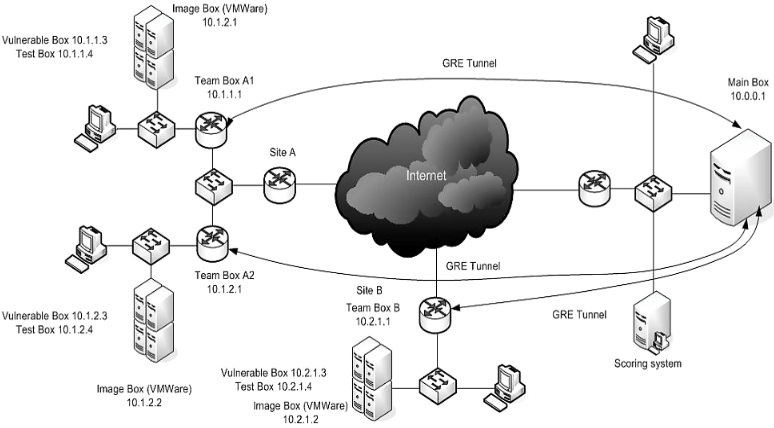
\includegraphics[width=0.9\textwidth]{inc/img/ad}
  \caption{Схема игровой сети UCSB CTF}
  \label{fig:ad}
\end{figure}

Примерная продолжительность такой игры --- от пяти до двенадцати часов. Победителей определяют по сумме баллов, набранных за всю игру.

Соревнования вида attack-defense требовательны к участникам. Для игры базово необходимо обладать следующими навыками и умениями:
\begin{enumerate}
  \item серверное администрирование для настройки и запуска игровых сервисов и конфигурации вулнбоксов;
  \item сетевые технологии для понимания поверхности атак, свзянанных с протоколами, а также для того, чтобы перехватывать трафик (одна из стратегий игры --- наблюдать, как другие команды эксплуатируют уязвимости и как можно быстрее повторять их действия\cite{ReplayAttacks});
  \item быстрое чтение программного кода сервисов, который может быть написан на любом языке программирования: от Python\cite{PythonService} до Haskell\cite{HaskellSerivce} или Bash\cite{BashService};
  \item и т.п.
\end{enumerate}




\subsection{Jeopardy CTF}

Этот вид CTF-соревнований отличается, в первую очередь, более простым набором правил, а также подходом: команды решают задачи, а не атакуют друг друга. Общие положения:

\begin{enumerate}
  \item Участникам предлагается одинаковый набор задач \textit{(англ. challenges)}.
  \item Каждая задача имеет описание, категорию, к которой она относится (см. табл. \ref{tab:categories}), а также стоимость.
  \item Решение каждой задачи подразумевает поиск и сдачу жюри одного флага. За сданный флаг команда получает столько очков, сколько стоило задание.
  \item В конце соревнований подводят итоги. Побеждают команды, первыми набравшие наибольшее число очков.
\end{enumerate}

\begin{figure}
  \centering
  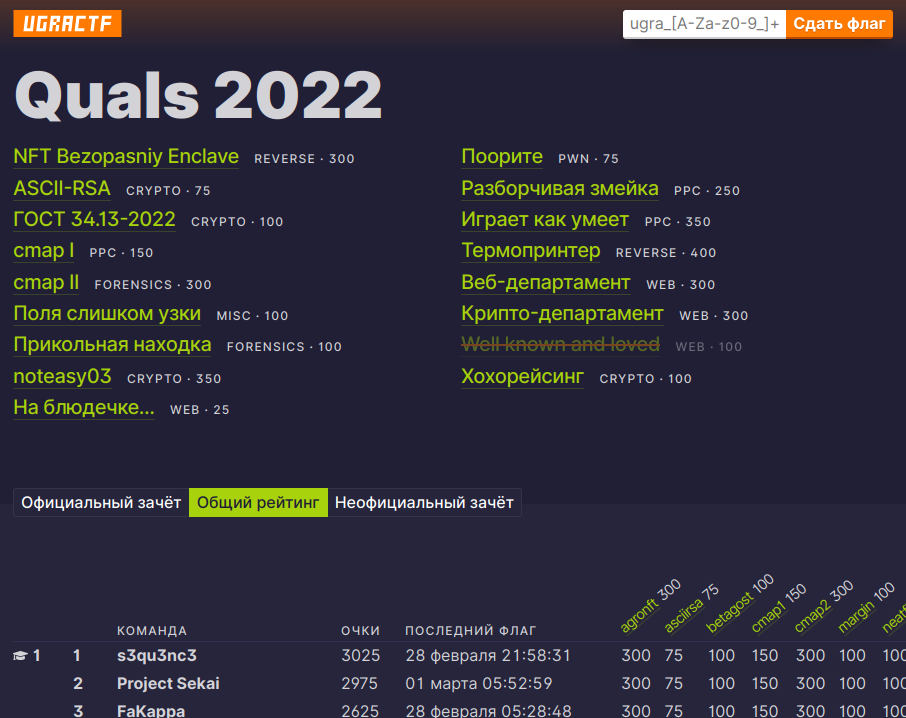
\includegraphics[width=0.5\textwidth]{inc/img/jeopardy}
  \caption{Главная страница игровой системы Ugra CTF}
  \label{fig:jeopardy}
\end{figure}


Своё название данный вид соревнований получил благодаря схожести с форматом телепередачи «Своя игра», в которой игроки выбирают вопросы, сгруппированные по темам и стоимости, с той лишь разницей, что в CTF команды решают задачи асинхронно и не должны видеть решения других команд. Таким образом, соревнования вида jeopardy больше похожи на соревнования по спортивному программированию, где участники получают баллы за верно решённые формально описанные задачи и дисквалифицируются за нечестную игру: списывание или получение иной внешней помощи.

Однако, формат CTF, ввиду своей специфики, даёт больше творческой свободы как составителям задач, так и решающим их людям. В частности, на CTF-соревнованиях --- даже школьных олимпиадах --- разрешается пользоваться интернетом и справочной литературой, поскольку, с одной стороны, решение может требовать от участников способности оперативно разобраться в новой, незнакомой технологии и проэксплуатировать её уязвимости, а с другой, задачи в CTF составляются так, чтобы быть не похожими на уже существующие. Последнему факту способствует важная традиция, принятая в сообществе: как организаторы, так и участники, после окончания соревнований, публикуют в открытом доступе т. н. «райтапы» \textit{(англ. writeup)} --- разборы решений задач. По этой же причине CTF-задачи за редким исключением (в случае закрытых соревнований внутри компаний либо некомпетентности организаторов) не переиспользуются в нескольких соревнованиях.

В отличие от attack-defense, порог входа в соревнования, построенные по принципам jeopardy, существенно ниже. Обычно участникам, чтобы получить доступ к игре, достаточно лишь зарегистрироваться в игровой системе. Из этого не следует, что задачи в jeopardy проще, чем эксплуатация уязвимостей сервисов в attack-defense. Для решения могут пригодиться самые разные умения и навыки. Именно поэтому задачи разделяют на категории, а команды зачастую состоят из специлаистов в непересекающихся областях.

\begin{center}
  \begin{longtable}{|p{0.12\textwidth}|p{0.82\textwidth}|}
    \caption{Некоторые категории CTF-задач}
    \label{tab:categories}
    \\ \hline
    Название & Пояснение
    \\ \hline \endhead
    \texttt{crypto}   & Криптография: задачи о слабых криптоалгоритмах \\
    \texttt{stegano}  & Стеганография: искусство тайной передачи информации \\
    \texttt{osint}    & Разведка по открытым источникам: поиск информации в интернете \\
    \texttt{ppc}      & Программирование: необходимо что-то автоматизировать \\
    \texttt{reverse}  & Реверс-инжиниринг: анализ бинарных файлов или работы программ \\
    \texttt{web}      & Веб-техологии: браузерные и серверные уязвимости \\
    \texttt{network}  & Компьютерные сети \\
    \texttt{admin}    & Администрирование: знание ОС и ПО \\
    \texttt{hardware} & Аппаратные устройства: микроконтроллеры, электротехника и т.п. \\
    \hline
  \end{longtable}
\end{center}

\Abbrev{ОС}{Операционная система}
\Abbrev{ПО}{Программное обеспечение}

Данная работа посвящена разработке среды для проведения соревнований по защите информации именно этого вида.




\section{Соревнования по защите информации Ugra CTF}
\label{cha:analysis:ugractf}

На момент написания данной ВКР автор проходит практику в Югорском научно-исследовательском институте информационных технологий. При поддержке этого института, а также по инициативе Департамента информационных технологий и цифрового развития Ханты-Мансийского автономного округа — Югры, в России с 2016 проводятся соревнования по защите информации Ugra CTF. Традиционно они проводились в два этапа: дистанционный отборочный для всех желающих и очный заключительный (финал) для лучших игроков, проводившийся в столице ХМАО, Ханты-Мансийске. Как правило, оба этапа представляли собой CTF вида jeopardy.

\begin{figure}
  \centering
  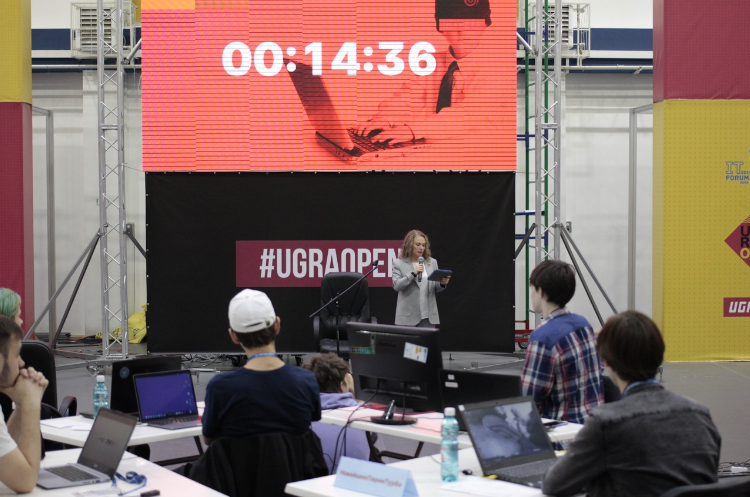
\includegraphics[width=0.6\textwidth]{inc/img/ugractf-19}
  \caption{Открытие Ugra CTF Finals 2019. 10 июня 2020 года, Ханты-Мансийск}
  \label{fig:ugractf-19}
\end{figure}

\Abbrev{ХМАО-Югра}{Ханты-Мансийский автономный округ — Югра}

В 2019–2020 году в состав организаторов вошёл Департамент образования и молодежной политики ХМАО-Югры. Примерно в это же время в России стало наблюдаться снижение числа регулярных CTF-соревнований для школьников. По разным причинам прекратили свою деятельность организаторы соревнований UfoCTF\cite{UfoCTF} и QCTF\cite{QCTF}, основных российских соревнований для новичков. В связи с этим, были внесены изменения в схему проведения соревнований — для школьников с 2021 года проводится отдельный т.н. \textit{распределённо-очный} индивидуальный (вместо командного) заключительный этап по правилам Российского совета олимпиад школьников.

\Abbrev{РСОШ}{Российский совет олимпиад школьников}

Соблюдение правил РСОШ в необходимо для включения соревнований Ugra CTF в государственный перечень школьных олимпиад. Это позволит победителям получать привилегии при поступлении в высшие учебные заведения. Однако, новый формат соревнований означает новые технические и организационные вызовы. Распределённо-очный заключительный этап --- компромисс между:
\begin{enumerate}
  \item полностью дистанционным проведением олимпиады, запрещённым правилами РСОШ ввиду отсутствия возможности контролировать участинков;
  \item полностью очным проведением, когда все участники собираются на единой площадке, полностью контролируемой оргкомитетом.
\end{enumerate}

При таком формате соревнования проходят в разных городах на разных площадках, предоставляемых партнёрами оргкомитета: частными фирмами, образовательными организациями или муниципалитетами. У оргкомитета сохраняется частичный контроль над инфраструктурой --- рабочими станциями участников, которые предоставляются площадками. Каждая площадка также выделяет из своих сотрудников наблюдателей, по совместительству вынужденных выолнять роль системных администраторов, что и вызывает основные сложности.

Соревнования компьютерные: от программного и аппаратного оснащения рабочих станций участников зависит многое. Зачастую требуются привилегированный доступ к системе и специализированные программные инструменты; к тому же дополнительные трудности могут возникать и в свете того, что многие игроки не используют наиболее распространённую в России ОС Windows, предпочитая UNIX-подобные системы как более подходящие для нетривиальных экспериментов, необходимых для решения многих игровых задач.

Настройка инфраструктуры, и контроль за соблюдением порой неочевидных правил требует определённой подготовки наблюдателей, которую оргкомитет по ряду причин не может осуществлять.

Таким образом, существует высокий риск того, что игра пройдёт с нарушениями. Например, согласно правилам РСОШ переговоры участников и получение внешней запрещены, однако, ввиду специфики соревнований пользоваться интернетом школьникам разрешается. Возникает закономерный вопрос: как отличить легитимное использование сети от тщательно замаскированной попытки опубликовать решение и получить помощь третьего лица?

В отборочном этапе 2021 года приняли участие 233 школьника в составе 93 команд. Помимо этого, более 450 команд со всего мира выполняли задания олимпиады в неофициальном зачёте \cite{Ugra21}. В том же этапе, но в 2022 году, приянло участие уже 383 школьника из 159 команд. Из них более 30 прошли в финал.

Для того, чтобы все финалисты смогли принять участие, команде разработки необходимо будет предоставить несколько десятков особым образом настроенных рабочих станций: от Санкт-Петербурга до Владивостока, и обеспечить бесперебойность работы всей инфраструктуры соревнований.



\section{Техническая архитектура соревнований}

Для проведения соревнований Ugra CTF необходима комплексная архитектура, которая позволит решить следующие задачи:

\begin{enumerate}

\item обеспечение решения игровых задач, включая получение условий, приём, валидацию и проверку флагов;
\item

\end{enumerate}

\Abbrev{TCP}{transmission control protocol --- протокол управления передачей}

\subsection{Система, обеспечивающая решение игровых задач}

Соревнования вида jeopardy с самого начала были автоматизированы. Это связано с относительно более тривиальным игровым процессом, чем в соревнованиях вида attack-defense. Обычно участники получают доступ к веб-приложению, которое содержит условия задач, турнирную таблицу и форму для сдачи флага. Его принято называть бордой.

\Define{борда}{\textit{(англ. board, буквально «доска»)} --- программная платформа для получения условий задач и сдачи флагов в CTF-соревнованиях вида jeopardy.}


\subsubsection{Требования к системе}

Борда должна отвечать ряду требований.

\begin{enumerate}

\item
В первую очередь, к таким требованиям можно отнести устойчивость к высоким нагрузкам. В отличие от соревнований вида attack-defense, где нагрузка команды атакуют друг друга (отношение «многие ко многим»), в jeopardy участники взаимодействуют с централизованной игровой инфраструктурой организаторов (отношение «многие к одному»). Отказ в обслуживании со стороны игровой платформы категорически недопустим, поскольку он создаёт неравные условия для игроков: возможна ситуация, когда часть участников успеет получить условие задачи или сдать флаг, в то время как другая --- нет.

Основные операции в платформе должны выполняться быстро и без существенных задержек. Желательно, чтобы система поддерживала многопоточную обработку пользовательских запросов там, где это возможно.

\item
Многопоточность, однако, зачастую приводит к неопределённости параллелизма. Эта неопределённость может послужить причиной ошибок: двойному начислению баллов, списанию некорректной суммы баллов при взятии подсказок или достижению некорректного состояния системы.

\Define{Неопределённость параллелизма}{ошибка проектирования многопоточной системы или приложения, при которой работа системы или приложения зависит от того, в каком порядке выполняются части кода}

\item
Тот факт, что соревнования --- по защите информации, накладывают повышенные требования к безопасности платформы. Не смотря на то, что правилами Ugra CTF запрещены атаки на инфраструктуру, непосредственно не относящуюся к игровым задачам, попытки вывести её из строя всё равно предпринимаются. Система должна быть устойчивой к наиболее распространённым веб-уязвимостям (обработка запросов, контроль пользовательских сессий и проч.), а также вести аудит всех событий для своевременного обнаружения оргкомитетом новых угроз.

\item
Платформа должна позволять обнаружать не только технические угрозы, но и более «человеческие»: пресекать попытки списывания, обмена участников флагами, решения соревнований одним и тем же лицом с нескольких аккаунтов (т.е. мультиаккаунтинг).

\item
Наконец, система должна быть гибкой. CTF --- творческий формат, поэтому структура и принципы могут меняться от игры к игры. Так, отборочный этап Ugra CTF 2019 представлял собой не простой jeopardy, где участникам сразу доступны все задания, а модельный тест на проникновение: сперва игрокам доступна лишь одна точка входа в вымышленную уязвимую систему. По мере «погружения» влубь этой системы открывались новые задания, которые выстраивались в нелинейную древовидную структуру\cite{UgraCTF19Q}.
\end{enumerate}


\subsubsection{Анализ существующих решений}

Существует множество программных продуктов, позволяющих проводить jeopardy -- CTF-соревнования, что называется, «под ключ»: организаторам необходимо лишь собрать участников, разработать задания и загрузить их на готовую платформу, при необходимости изменив некоторые её параметры. К сожалению, автору не удалось обнаружить такой системы, которая удовлетворяла бы всем требованиям \textit{(а)---(д)}, данным выше (табл. \ref{tab:boards}).

\begin{center}
  \begin{longtable}{|p{0.26\textwidth}|p{0.15\textwidth}|p{0.25\textwidth}|c|c|c|c|c|}
    \caption{Сравнительный анализ наиболее популярных готовых jeopardy-платформ}
    \label{tab:boards}
    \\ \hline
    \multirow{2}{*}{Название} & \multirow{2}{*}{Лицензия} & \multirow{2}{*}{Комментарий} & \multicolumn{5}{c|}{Требования} \\ \cline{4-8}
                              &                           &                              & (а) & (б) & (в) & (г) & (д) \\
    \hline \endhead
    ctfd                  & Коммерческая & \small{Непроизводительная}                     & − & ? & + & + & ± \\
    \hline
    yatb                  & Apache       &                                                & + & + & + & ? & − \\
    \hline
    Google kCTF           & Apache       & \small{Крайне сложная архитектура}             & + & + & + & − & − \\
    \hline
    Google CTF Scoreboard & Apache       & \small{Не развивается с 2018     }             & + & + & + & − & − \\
    \hline
    FBCTF                 & CC-BY-NC     & \small{Не развивается с 2018, нет аудита     } & + & + & − & + & − \\
    \hline
    picoCTF               & MIT          & \small{Не развивается с 2019     }             & − & − & + & − & − \\
    \hline
    mellivora             & GPLv3        & \small{Написана на PHP           }             & − & − & − & − & − \\
    \hline
  \end{longtable}
\end{center}

\chapter*{Выводы к Главе 1}

Вывод.


%%% Local Variables:
%%% mode: latex
%%% TeX-master: "rpz"
%%% End:

% \chapter{Теоретическая часть}

\section{Условия проведения оилмпиады Ugra CTF}

Большую часть задач, связанных с проведением школьной олимпиады по защите информации Ugra CTF, можно автоматизировать.

В первую очередь, для этого необходимо разработать формальное описание задач с учётом специфики олимпиады Ugra CTF. Существует ряд требований, который необходимо удовлетворить: внутренние и внешние.

Источников внутренних требований несколько. К ним относятся официальные нормативные документы: положение об олимпиаде и регламент её проведения. Среди них наиболее важен регламент. Именно в нём описаны:

\begin{itemize}
\item порядок регистрации участников,
\item порядок проведения этапов олимпиады,
\item правила оформления и проверки работ,
\item порядок подведения итогов и др.
\end{itemize}

Эти требования составлены с учётом общих принципов проведения CTF-соревнований вида Jeopardy и уже написаны формальным языком. Кроме того, поскольку требования внутренние, их допустимо видоизменять.

Ко внешним требованиям относится «Порядок проведения олимпиад школьников», документ, написанный РСОШ и утверждённый приказом Министерства образования и науки РФ. Этот документ, в частности, описывает общие положения и то, как должна проходить олимпиада. Большая часть требований РСОШ уже включена во внутренный регламент проведения олимпиады, и эти требования видоизменять нельзя.

Следует отметить, что большая часть требований носит скорее юридический характер, и практически не устанавливает требования к технической инфраструктуре. Поэтому, их необходимо будет составить самостоятельно.

Кроме нормативно-правовых актов, регулирующих порядок проведения олимпиады и требования к участникам, существуют физические и технические ограничения, связанные с распределённо-очным форматом проведения олимпиады. Например, несмотря на сравнительную популярность CTF-соревнований, нельзя ожидать, что наблюдатели на площадках будут знакомы с особенностями этого формата и способны самостоятельно сконфигурировать подходящее сетевое и программное окружение для участников.

\subsection{Правила и порядок проведения олимпиады Ugra CTF}

Олимпиада состоит из двух этапов: отборочного (отбора, Ugra CTF Quals) и заключительного (финала, Ugra CTF School).

Отборочный этап проводится в дистанционном формате и состоит из двух зачётов. К участию в официальном зачёте допускаются обучающиеся школ и средне-специальных учебных организаций (колледжей, училищей и т.д.). Неофициальный зачёт открыт для всех желающих без ограничений, но такого права не даёт. Отоборочный этап командный — в составе команды может быть от 1 до 5 человек.

Победители и призёры официального зачёта отборочного этапа олимпиады получают право на прохождение в заключительный этап. Заключительный этап, как отмечалось в §\ref{cha:analysis:ugractf}, проводится в распределённо-очном формате — участникам необходимо очно присутствовать на площадке. Заключительный этап индивидуальный — каждый участник решает задачи самостоятельно.

Оба этапа проходят по похожему принципу. Зарегистрировавшиеся участники получают доступ к проверяющей системе — сайту олимпиады — на котором размещены задачи и форма для сдачи ответов. Ответом к каждому заданию является флаг — строка, удовлетворяющая регулярному выражению \texttt{ugra[A-Za-z0-9\_]\{2,\}}, например, \texttt{ugra\_ex4mpl3}.

\Define{Регулярное выражение}{текстовая строка особого формата, задающая конечный автомат для поиска определённой подстроки или подстрок в тексте}

В соответствии с принципами проведения CTF-соревнований в формате Jeopardy, за сданные в проверяющую систему флаги команда получает столько баллов, сколько стоило каждое задание. Побеждают команды, набравшие наибольшее количество баллов. При равенстве баллов побеждает команда, быстрее решившая последнее задание.

По внутренним правилам олимпиады, на всех этапах запрещены следующие действия:
\begin{enumerate}
\item атака на инфраструктуру соревнований, к которой относятся, например, сервера, на которых размещена проверяющая система и задачи;
\item обмен условиями задач, если этот обмен не происходит между участниками одной команды во время отборочного этапа — в заключительном этапе этого исключения нет по причине индивидуального характера соревнований;
\item обмен флагами.
\end{enumerate}

Важно также соблюдать принцип равенства всех участников: никто не должен обладать преимуществом. Преимуществом можно считать как получение внешней помощи, например, путём публикации условий задач на интернет-форуме, так и ситуацию, в которой одной команде на решение было дано больше времени, чем другой — приём проверяющей системой флагов должен прекращаться одновременно для всех участников точно в момент окончания соревнований.

РСОШ требует предоставлять подробную отчётность об организации и проведении олимпиад, а также их результатах. В эту отчётность должны входить работы участников — в контексте CTF ими являются флаги, причём, неверные посылки также должны быть отражены в отчёте.

\subsection{Подход к построению системы проведения испытаний}

Требования к проведению отборочного этапа олимпиады в обобщённом виде есть подмножество требований к проведению заключительного этапа. Следовательно, при грамотном системном подходе к проектированию и разработке такой системы, можно ориентироваться только на более обширные и строгие требования финала.

Из требований финала — как юридических, так и технического характера, и учитывая распределённо-очный формат проведения этого этапа, следует, что система должна способствовать решению следующих основных задач:

\begin{itemize}
\item управлять материалами соревнований и работами участников;
\item предоставлять очным участникам программную среду для решения задач;
\item контролировать ход проведения соревнований.
\end{itemize}

Это большой работы на пересечении многих областей. Разумно предположить, что при подробной декомпозиции этих задач может выясниться, что для каких-то подзадач уже существуют готовые решения. Использование готовых решений — будь то программный продукт или аппаратный комплекс — позволяет снизить стоимость разработки системы.

Значит, к решению этих задач следует подходить, разработав не единую систему, а комплекс из разделённых подсистем, взаимодействующих между собой. При таком подходе, как правило, получаются модульные и гибкие системы, что желательно в данном случае — правила отбора и финала отличаются, требования РСОШ из года в год меняются, форматы CTF эволюционируют. Стоит предусмотреть возможность масштабирования и устойчивости системы в изменчивых условиях.


\section{Система управления материалами соревнований и работами участников (борда)}

Первые CTF-соревнования проводились практически полностью вручную. Так, участники первых DEF CON CTF отправляли флаги оргкомитету в текстовом чате. Со временем, стали появляться автоматизированные решения, которые автоматически генерировали флаги, размещали их в сервисах команд и принимали посылки участников по протоколу TCP.

\Abbrev{TCP}{(англ. transmission control protocol) — сетевой протокол транспортного уровня, используемый для передачи данных с подтверждением получения.}

Соревнования вида jeopardy с самого начала были автоматизированы. Это связано с относительно более тривиальным игровым процессом, чем в соревнованиях вида attack-defense. Обычно участники получают доступ к веб-приложению, которое содержит условия задач, турнирную таблицу и форму для сдачи флага. Его принято называть \textit{бордой.}

\Define{борда}{\textit{(англ. board, буквально «доска»)} --- программная платформа для получения условий задач и сдачи флагов в CTF-соревнованиях вида jeopardy.}


\subsection{Организационные требования к системе}

Внутренний регламент проведения олимпиады и положение РСОШ предъявляют большое число требований к тому, каким образом участникам выдаются материалы (задачи) и оцениваются работы.

Борда должна содержать все условия опубликованных задач. Допускается публикация новых задач после начала мероприятия и изменение условий уже опубликованных, если они содержат ошибки.

Борда отвечает за проверку решений участников — валидацию флагов. Валидация должна осуществляться безошибочно, ответы участников, вне зависимости от их верности, необходимо фиксировать для отчётности. Приём решений должен начинаться и заканчиваться одновременно для всех участников вместе с, соответственно, началом и окончанем соревнований.

Желательно, чтобы в борде был предусмотрен механизм, позволяющий определять, самостоятельно ли участник получил флаг. Это позволит обеспечить более тщательный контроль за соблюдением соответствующего правила в положении РСОШ. Частично это достигается путём реализации системы, генерирующей задачи «по вариантам»: с общим принципом решения, но уникальным для каждого участника ответом. В этом случае любая попытка недобросовестной сдачи участником флага, ему не предназначенного, автоматически считается неверной и обнаруживается тривиальным образом.

\subsection{Технические требования к системе}

Борда должна отвечать ряду требований.

\begin{enumerate}

\item
В первую очередь, к таким требованиям можно отнести устойчивость к высоким нагрузкам. В отличие от соревнований вида attack-defense, где нагрузка команды атакуют друг друга (отношение «многие ко многим»), в jeopardy участники взаимодействуют с централизованной игровой инфраструктурой организаторов (отношение «многие к одному»). Отказ в обслуживании со стороны игровой платформы категорически недопустим, поскольку он создаёт неравные условия для игроков: возможна ситуация, когда часть участников успеет получить условие задачи или сдать флаг, в то время как другая --- нет.

Основные операции в платформе должны выполняться быстро и без существенных задержек. Желательно, чтобы система поддерживала многопоточную обработку пользовательских запросов там, где это возможно.

\item
Многопоточность, однако, зачастую приводит к неопределённости параллелизма. Эта неопределённость может послужить причиной ошибок: двойному начислению баллов, списанию некорректной суммы баллов при взятии подсказок или достижению некорректного состояния системы.

\Define{Неопределённость параллелизма}{ошибка проектирования многопоточной системы или приложения, при которой работа системы или приложения зависит от того, в каком порядке выполняются части кода}

\item
Тот факт, что соревнования --- по защите информации, накладывают повышенные требования к безопасности платформы. Не смотря на то, что правилами Ugra CTF запрещены атаки на инфраструктуру, непосредственно не относящуюся к игровым задачам, попытки вывести её из строя всё равно предпринимаются. Система должна быть устойчивой к наиболее распространённым веб-уязвимостям (обработка запросов, контроль пользовательских сессий и проч.), а также вести аудит всех событий для своевременного обнаружения оргкомитетом новых угроз.

\item
Наконец, система должна быть гибкой. CTF --- творческий формат, поэтому структура и принципы могут меняться от игры к игры. Так, отборочный этап Ugra CTF 2019 представлял собой не простой jeopardy, где участникам сразу доступны все задания, а смоделированный в виде иерархического дерева задач тест на проникновение в корпоративную систему вымышленного банка. Сперва игроку доступна лишь точка входа --- сайт организации; по мере изучения системы открываются новые задачи, причём, какая именно задача откроется следующей, зависит от набора уже решённых\cite{UgraCTF19Q}.
\end{enumerate}


\subsection{Анализ существующих решений}

\begin{figure}
  \centering
  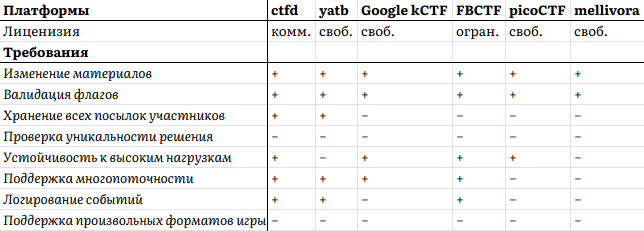
\includegraphics[width=0.9\textwidth]{inc/img/boards-table}
  \caption{Таблица 2.1. Сравнительный анализ наиболее популярных платформ для Jeopardy CTF}
  \label{fig:jeopardy}
\end{figure}

Существует множество программных продуктов, позволяющих проводить jeopardy -- CTF-соревнования: организаторам необходимо лишь собрать участников, разработать задания и загрузить их на готовую платформу.

Анализ наиболее популярных готовых проверяющих систем для Jeopardy CTF показал, что ни одна такая система не удовлетворяет всем необходимым требованям (табл. 2.1). Выборка состоит из трёх систем, наиболее популярных на ресурсе Github\cite{GithubCTFTag} по тегу «ctf board» (yatb, picoCTF, mellivora), а также трёх систем, которые используются для проведения наиболее популярных международных соревнований по статистике агрератора CTFTime.org\cite{CTFTime}.

\section{Генерация вариантов задач и их развёртывание}

Обычно размещают задачи и следят за их работоспособностью вручную — можно автоматизировать этот процесс. Задачи часто однотипны с инфраструктурной точки зрения: это или веб-приложения, или сервисы на сокетах, или сгенерированные автоматически файлы. Можно разработать систему, позволяющую декларативно описать, как устроена задача, и делегировать полномочия по её развёртыванию борде.

Это же поможет реализовать более защиту от списывания: генерировать каждой команде по своему собственному варианту задачи со своим собственным флагом. Даже если задача статическая (например, на криптографический анализ текста).

Реализовать такой механизм можно, реализовав программный интерфейс для запуска задач. Конфигурация конкретной задачи описывается на формальном языке.

Для развёртывания статических задач борде передаётся т.н. генератор — программа, криптографическими методами генерирующая флаг задачи для конкретного участника, условие и файлы-вложения, если они есть.

Для развёртывания динамических задач борде, помимо генератора, передаётся инструкция по запуску процесса, тому, на каком домене или адресе он должен быть доступен, и при каких условиях его необходимо перезапустить или остановить.

Генерация варианта задачи может оказаться ресурсоёмким процессом. Для таких случаем необходимо предусмотреть возможность предварительной генерации определённого числа вариантов, когда нагрузка на инфраструктуру минимальна (например, до начала соревнований) с кешированием результатов и распределением между участниками по мере их появления.

\subsection{Система, предоставляющая очным участникам программную среду для решения задач}

Каждому участнику на площадке предоставляется компьютер.

Программная среда компьютера должна быть пригодной для решения CTF-задач: нужен Linux с правами администратора (чтобы устанавливать своё ПО, изменять конфигурацию системы и т.п.).

Поскольку компьютеры не наши, жёсткий диск лучше не трогать.

Следовательно, среду лучше записывать на внешний загрузочный носитель — причём, участнику давать доступ к виртуальной машине, а в родительской ОС разместить инструменты прокторинга и провизии.

Использование виртуальной машины подразумевает наличие какого-то образа ОС. Поскольку это непринциаильный момент, можно предусмотреть возможность участника, при его желании, использовать свой образ ОС, а также поставлять универсальный «нейтральный» образ любого подходящего дистрибутива ОС Linux. Например, Kali Linux — наиболее распространённый дистрибутив, в комплекте поставки которого содержится большое количество инструментов для исследования уязвимостей.

Таким образом, можно сформулировать требования к функциональности такой системы.

\begin{enumerate}
\item Автоматически разворачивается виртуальная машина с образом ОС, заблаговременно предоставленным участником через свой личный кабинет;
\item Все остальные приложения полностью изолируются от участника;
\item Реализованы элементы прокторинга: периодически с машины каждого участника собираются скриншоты, которые в перспективе планируется автоматически анализировать на предмет нарушения правил — там всё неочевидно, поскольку мы разрешаем пользоваться интернетом, но запрещаем любую внешнюю помощь и распространение условий задач;
\item Настраивается сетевой тоннель в общую игровую сеть;
\item Обеспечивается возможность удалённого доступа организаторов к любой машине;
\item Гарантируется невозможность модификации запущенной хост-ОС: её системных файлов, конфигурации ПО и пользователей с группами.
\end{enumerate}

Прокторинг:
\begin{itemize}
\item
  запись экрана;
\item
  контроль целостности ОС.
\end{itemize}

Провизия:
\begin{itemize}
\item
  участники могут работать в любой ОС, образ которой заблаговременно предоставят, либо в стандартом окружении Kali Linux (вариант по умолчанию);
\item
  конфигурация сети;
\item
  вывод на рабочем столе сведений об участниках («подписать», где чей компьютер);
\item
  возможность удалённого доступа к каждой машине для администрирования.
\end{itemize}


\section{Общая модель системы}

\subsection{Модель компьютерной системы}

\begin{itemize}
\item
  сервер жюри с бордой (веб-интерфейс, HTTPS);
\item
  сервер провизии и прокторинга (управление через SSH);
\item
  хранилище образов ВМ участников;
\item
  рабочие места участников.
\end{itemize}

\section{Модель угроз}

\subsection{Модель нарушителя}

Участник:
\begin{itemize}
\item
  может общаться в интернете
\item
  может обмениваться флагами с другими участниками
\item
  может обмениваться условиями задач с внешним миром
\item
  может атаковать инфраструктуру (в разных местах)
\end{itemize}

Организатор:
\begin{itemize}
\item может помогать участникам
\item может получить доступ к условиям задач
\item может не пресекать нарушения правил
\end{itemize}

%\chapter{РАЗРАБОТКА ПРОГРАММНОЙ СРЕДЫ}



\section{Итоговая архитектура среды}

Прежде чем приступить к разработке среды, подробно опишем её компоненты, связи между этими компонентами и соответствующией функции.

Среда~--- это программная система, которая состоит из двух основных модулей. Чтобы различать их, перечислим их и присвоим каждому название:
\begin{itemize}
\item модуль управления ходом испытания \textit{Kyzylborda\footnotemark[1];}
\item модуль, предоставляющий участникам среду для прохождения испытаний \textit{SchoolOS}.
\end{itemize}

\footnotetext[1]{Название системы придумано другим членом оргкомитета и является каламбуром: с одной стороны, этот модуль реализует то, что называют словом <<борда>>, с другой~--- существует известный казахстанский город Кызылорда, и эти слова рифмуются. Упустить такой шанс было невозможно.}
\Abbrev{HTTP}{(англ. hypertext transfer protocol) протокол передачи гипертекста}
\Abbrev{UML}{(англ. unified modeling language) единый язык для моделирования}

Архитектуру среды можно описать на языке диаграмм UML \textit{(англ. unified modeling language, единый язык для моделирования).} UML~--- это открытый стандарт, позволяющий создавать графическое представление сложных систем на разных уровнях: от глобального межсистемного взаимодействия до локальных сценариев использования конкретных компонент \cite{UML}.

Для описания архитектуры была составлена т.н. диаграмма пакетов (рисунок \ref{fig:uml-model}), отражающая связи между произвольными группами сущностей, объединёнными семантически, т.е. \textit{пакетами.} В данном случае в роли пакетов выступают системы и подсистемы среды. Пунктирными стрелками устанавливается отношение <<пакет зависит от>>: так устанавливаются абстрактные функциональные связи.

\Define{Пакет (в UML)}{механизм общего назначения в языке UML для группировки элементов по семантическим связям в целях обеспечения наглядности структуры модели системы}

\begin{figure}[h]
  \centering
  \includegraphics[width=1\textwidth]{inc/dia/uml-model.eps}
  \caption{UML-диаграмма пакетов для среды}
  \label{fig:uml-model}
\end{figure}

Модуль Kyzylborda~--- это клиент-серверное приложение с веб-интерфейсом, то есть приложение, доступ к которому осущесвтляется пользователями по протоколу HTTP \textit{(англ. hyptertext transfer protocol, протокол передачи гипертекста).} Оно состоит из модуля задач и модуля, предоставляющего веб-интерфейс.

Модуль SchoolOS~--- это дистрибутив ОС Linux, содержащий в себе клиент-серверные компоненты, реализующие функциональность, связанную с провизией и прокторингом, а также предоставляющий доступ участника к ВМ с гостевой ОС.

Пакеты этих модулей были декомпозированы с учётом функций, описанных в Главе 2. В ходе дальнейшей разработки декомпозиция будет продолжена.

Оба модуля так или иначе должны взаимодействовать с уже существующей ИС <<Юрт>>, используемой оргкомитетом для регистрации участников и обработки их персональных данных. Интеграция с ИС в случае модуля Kyzylborda необходима для обеспечения аутентификации участников, в случае SchoolOS~--- для получения сведений о них и о проводимом испытании.

Описание разработки модулей будет производиться в обратном порядке, чем в предыдущей главе. Это связано с тем, что технологию NixOS, используемую в обоих модулях, лучше начать рассматривать с примеров, связанных с её непосредственным назначением~--- управлением конфигурацией ОС, которые возникнут при разработке SchoolOS.

\FloatBarrier

\section{Модуль среды SchoolOS}

Технологическая основа для данного модуля~--- базовая операционная система. В Главе 2 для этой роли был выбран дистрибутив ОС Linux, NixOS, построенный вокруг функционального декларативного пакетного менеджера Nix.

NixOS позволяет описать состояние ОС целиком как будто это состояние~--- ещё один пакет, подлежащий установке. Такой подход позволяет обеспечить, во-первых~--- воспроизводимость сборки конфигурации, во-вторых~--- её неизменчивость (иммутабельность). Любые изменения, вносимые в конфигурацию применяются подобно транзакциям, порождая каждый раз новую версию ОС, а не производятся <<наживую>>, как это реализовано в традиционных пакетных менеджерах.

С помощью конфигурации NixOS можно определить системные параметры, включая параметры загрузки и настройки разграничения доступа, набор установленного ПО, (а также само ПО как пакет, если речь идёт о самостоятельно разработанных программах), перечень системных сервисов и прочие нюансы.

В предыдущем разделе отмечалось, что модули, обеспечивающие прокторинг и провизию, требуют клиент-серверной архитектуры, причём взаимодействие сторон должно осуществляться по протоколу SSH. NixOS позволяет также разработать и конфигурацию ОС для сервера, упростив и автоматизировав процесс его развёртывания в дальнейшем.

Сами модули для прокторинга и провизии стоит разработать как набор скриптов для командной оболочки ОС Linux, поскольку их реализация не подразумевает сложных алгоритмов, но требует постоянного взаимодействия с разными частями базовой ОС~--- напрмер, захват экрана, создание SSH-туннелей и т.п.

Таким образом, для имплементации модуля SchoolOS необходимо:
\begin{enumerate}
\item
  разработать модули провизии и прокторинга;
\item
  разработать конфигурацию NixOS для базовой ОС (клиент);
\item
  разработать конфигурацию NixOS для серверной ОС.
\end{enumerate}

\subsection{Подмодуль провизии и прокторинга}

Определим протокол взаимодействия клиента и сервера и способ соединения. Для целей провизии, центральному серверу необходимо получать актуальную и полную картину того, какие клиенты к нему подключены~--- это также следует предусмотреть при разработке подмодуля.

Кроме того, необходимо, чтобы провизия осуществлялась в ручном режиме на случай сбоев.

\subsubsection{Протокол клиент-серверного взаимодействия}

С помощью SSH можно выполнять команды на удалённой машине. При этом, открывается сеанс в командной оболчке пользователя, от имени которого осуществляется доступ.

Де-факто стандартная имплементация SSH, программа OpenSSH, позволяет изменить это поведение. Можно настроить сервер так, чтобы при подключении выполнялась одна и та же команда независимо от того, с каким запросом подключился клиент. То есть, если, например, указать в параметрах сервера следующую директиву \texttt{command="/bin/date"}, то при подключении к нему по SSH клиент получит только текущую дату, после чего программа завершится.

Этот механизм позволяет безопасно реализовать обработчик подключений. Более того, при работе в таком режиме, в окружение сервера передаётся переменная окружения \texttt{SSH\_ORIGINAL\_COMMAND}, из которой можно получить данные <<запроса>> клиента.

Клиенты должны однозначно идентифицироваться и содержать данные о пользователе, а также об испытании. Первая проблема решена за нас разработчиками ОС Linux: при первой загрузке она случайным образом генерирует 128-битовый уникальный идентификатор и записывает его в файл \texttt{/etc/machine\_id}. Этого идентификатора достаточно для наших целей.

Вторая проблема решается введением следующих данных, которые могут быть записаны в образе заранее либо получаться от сервера:

\begin{itemize}
\item \texttt{short\_id}: шифр (трёхзначное число, которое выдается каждому участнику согласно регламенту проведения олимпиады);
\item \texttt{long\_id}: фамилия и инициал участника (текстовая строка);
\item \texttt{tag}: метка, соответствующая площадке олимпиады, к которой относится компьютер.
\end{itemize}

Кажде значение будем хранить в отдельном файле в директории \texttt{/provision/}.

\subsubsection{Наблюдение за состоянием клиентов}

Уточним алгоритм из \S \ref{cha:ana:ssh}.

\begin{lstlisting}[language=python,caption={Алгоритм клиента (псевдокод)}]
    туннель := открыть туннель до сервера
    цикл:
        если туннель открыт:
            подключиться к серверу по SSH
            сообщить серверу (machine_id, порт туннеля)
            (short_id, long_id, tag) := получить от сервера
            если любой из (short_id, long_id, tag) /= системные значения:
                обновить системные значения на (short_id, long_id, tag)
            пауза 10 сек
        иначе:
            туннель := открыть туннель до сервера
\end{lstlisting}

Такой аглоритм по сути реализует механизм, подобный  KeepAlive из протокола TCP \cite{TCPKeepalive}: клиент и сервер договариваются о том, что соединение установлено, и клиент поддерживает его в открытом состоянии с той разницей, что используется не TCP-сокет.

На сервере будем хранить базу данных клиентов в текстовом формате JSON \cite{JSON}. Это распространённый формат, позволяющий хранить структурированные данные в виде списков и таблиц, для работы с которым разработаны инструменты и в Nix (функции стандартной библиотеки языка), и в Linux (утилита \texttt{jq}).

Реализуем SSH-интерфейс со следующим синтаксисом:

\begin{lstlisting}[caption={Синтаксис обработчика SSH-соединений для провизии}]
<command> := "get-info" <short-id>
           | "update"   <machine-id> <port> <tag>
\end{lstlisting}

Первая команда будет возвращать машиночитаемые значения индентификаторов, присвоенных машине, чтобы клиент мог записать их себе. Вторая~--- наоборот, принимать от клиента данные о себе и обновлять соответствующим образом базу данных.

\subsubsection{Онлайн-провизия}

Имея базу данных и сведения об адресах всех клиентов, тривиально написать скрипт, позволяющий присваивать любой машине необходимые значения \texttt{machine\_id}, \texttt{short\_id}, \texttt{tag}.

\begin{lstlisting}[caption={Скрипт \texttt{remote-customize.sh} для онлайн-провизии (отрывок)}]
# откроем файловый сокет для подключения к клиенту
ssh -fNMS "$tmpdir/sock" -o StrictHostKeyChecking=no -o UserKnownHostsFile=/dev/null -p "$port" root@127.0.0.1

# введём вспомогательную процедуру для обращения к клиенту
# посредством открытого сокета
callSsh() {
  ssh -S "$tmpdir/sock" placeholder "$@"
}

# создадим на клиенте директорию с данными провизии
callSsh -- mkdir -p /provision

# будем проверять данные, переданные скрипту
# и при их наличии записывать их в файлы на клиенте
if [ -n "$new_short_id" ]; then
  echo "$new_short_id" | callSsh -- sh -c "'cat > /provision/short-id'"
fi
# и так далее
\end{lstlisting}

\subsubsection{Ручная провизия}

Для ручной провизии достаточно получить права администратора в системе и самостоятельно изменить данные, содеражищеся в директории /provision/. Изменения применятся автоматически.

Образы гостевых ОС целесообразно размещать прямо на USB-накопителях со SchoolOS, поскольку они обладают размером от нескольких гигабайт, и передавать такие большие объёмы данных (с учётом того, что в среднем в финале участвует более сорока человек, и образ нужен каждому) через интернет проблематично, особенно учитывая, что далеко не на всех площадках скорость подключения позволяет это сделать быстро.

Необходим инструмент, позволяющий осуществлять провизию прямо на образ среды перед его записью на накопитель. Для этого существует программа Guestfish \cite{Guestfish}. Guestfish предоставляет shell-подобный интерфейс для работы с виртуальными файловыми системами дисковых образов. С помощью этой программы можно копировать, создавать и удалять файлы образа SchoolOS, задавая данные для провизии и записывая произвольный образ гостевой ОС.

\subsubsection{Прокторинг}

Для записи экрана участника воспользуемся утилитой \texttt{ffmpeg}. Она позволяет осуществлять захват экрана в видеопоток, а также кодировать его и сохранять в файл. Достичь необходимого результата можно, написав два скрипта: один для непосредственной записи экрана, второй~--- для оперативной передачи записей на сервер.

Они должны работать параллельно и в фоновом режиме, а также автоматически перезапускаться в случае возникновения ошибок. Кроме того, у участника не должно быть возможности прервать запись ни при каких обстоятельствах. Для этого для каждого скрипта можно создать соответствующий системный сервис~--- ОС предоставляет механизм для запуска, мониторинга и управления ходом работы произвольных процессов, который называется \texttt{systemd} \cite{Systemd}.

\subsection{Разработка конфигурации базовой операционной системы}

\subsubsection{Разграничение доступа}

В ОС Linux предусмотрена дискреционная система разграничения доступа с несколькими способами авторизации и аутентификации.

Каждый файл в файловой системе ОС обладает меткой, указывающей на права доступа: чтение, запись и исполнение. Метка содержит права доступа в трёх экземплярах: для владельца файла~--- пользователя системы, для группы пользователей, к которой относится владелец, а также права для всех остальных.

Настроим NixOS так, чтобы в системе содержалось три пользователя:
\begin{itemize}
\item \texttt{root}: суперпользователь для управления машиной;
\item \texttt{user}: непривилегированная учётная запись, в которой будет работать участник;
\item \texttt{schoolos-screencast}: учётная запись, в которой ведётся прокторинг.
\end{itemize}

Такая структура должна позволять участнику перезагружать компьютер и запускать виртуальную машину. И не должна позволять изменять данные провизии и останавливать системный сервис прокторинга, поскольку он запущен от другого лица.

\begin{lstlisting}[caption={Конфигурация разграничения доступа}]
users = {
  extraUsers = {
    root = {
      openssh.authorizedKeys.keyFiles = "..."; # SSH ключ оргкомитета
      hashedPassword = "..."; # пароль пользователя root
    };
    user = {
      isNormalUser = true;
      password = ""; # пустой пароль для user
      extraGroups = [ "vboxusers" ]; # право запускать ВМ
    };
    schoolos-screencast = {
      isSystemUser = true;
      group = "schoolos-screencast";
      home = "/var/lib/schoolos-screencast";
    };
  };
};
\end{lstlisting}

\subsubsection{Графическая индикация инициализации системы}

В числе требований, предъявленных к SchoolOS, была необходимость графической индикации инициализации системы. Для этого был разработан скрипт \texttt{wallpaper.py}, генерирующий графическое изображение, которое автоматически устанавливается в качестве фона рабочего стола.

Скрипт написан на языке программирования Python, использует для работы графическую библиотеку Pillow и системные вызовы ОС Linux, позволяющие автоматически определить текущее разрешение экрана.

\begin{figure}[h]
  \centering
  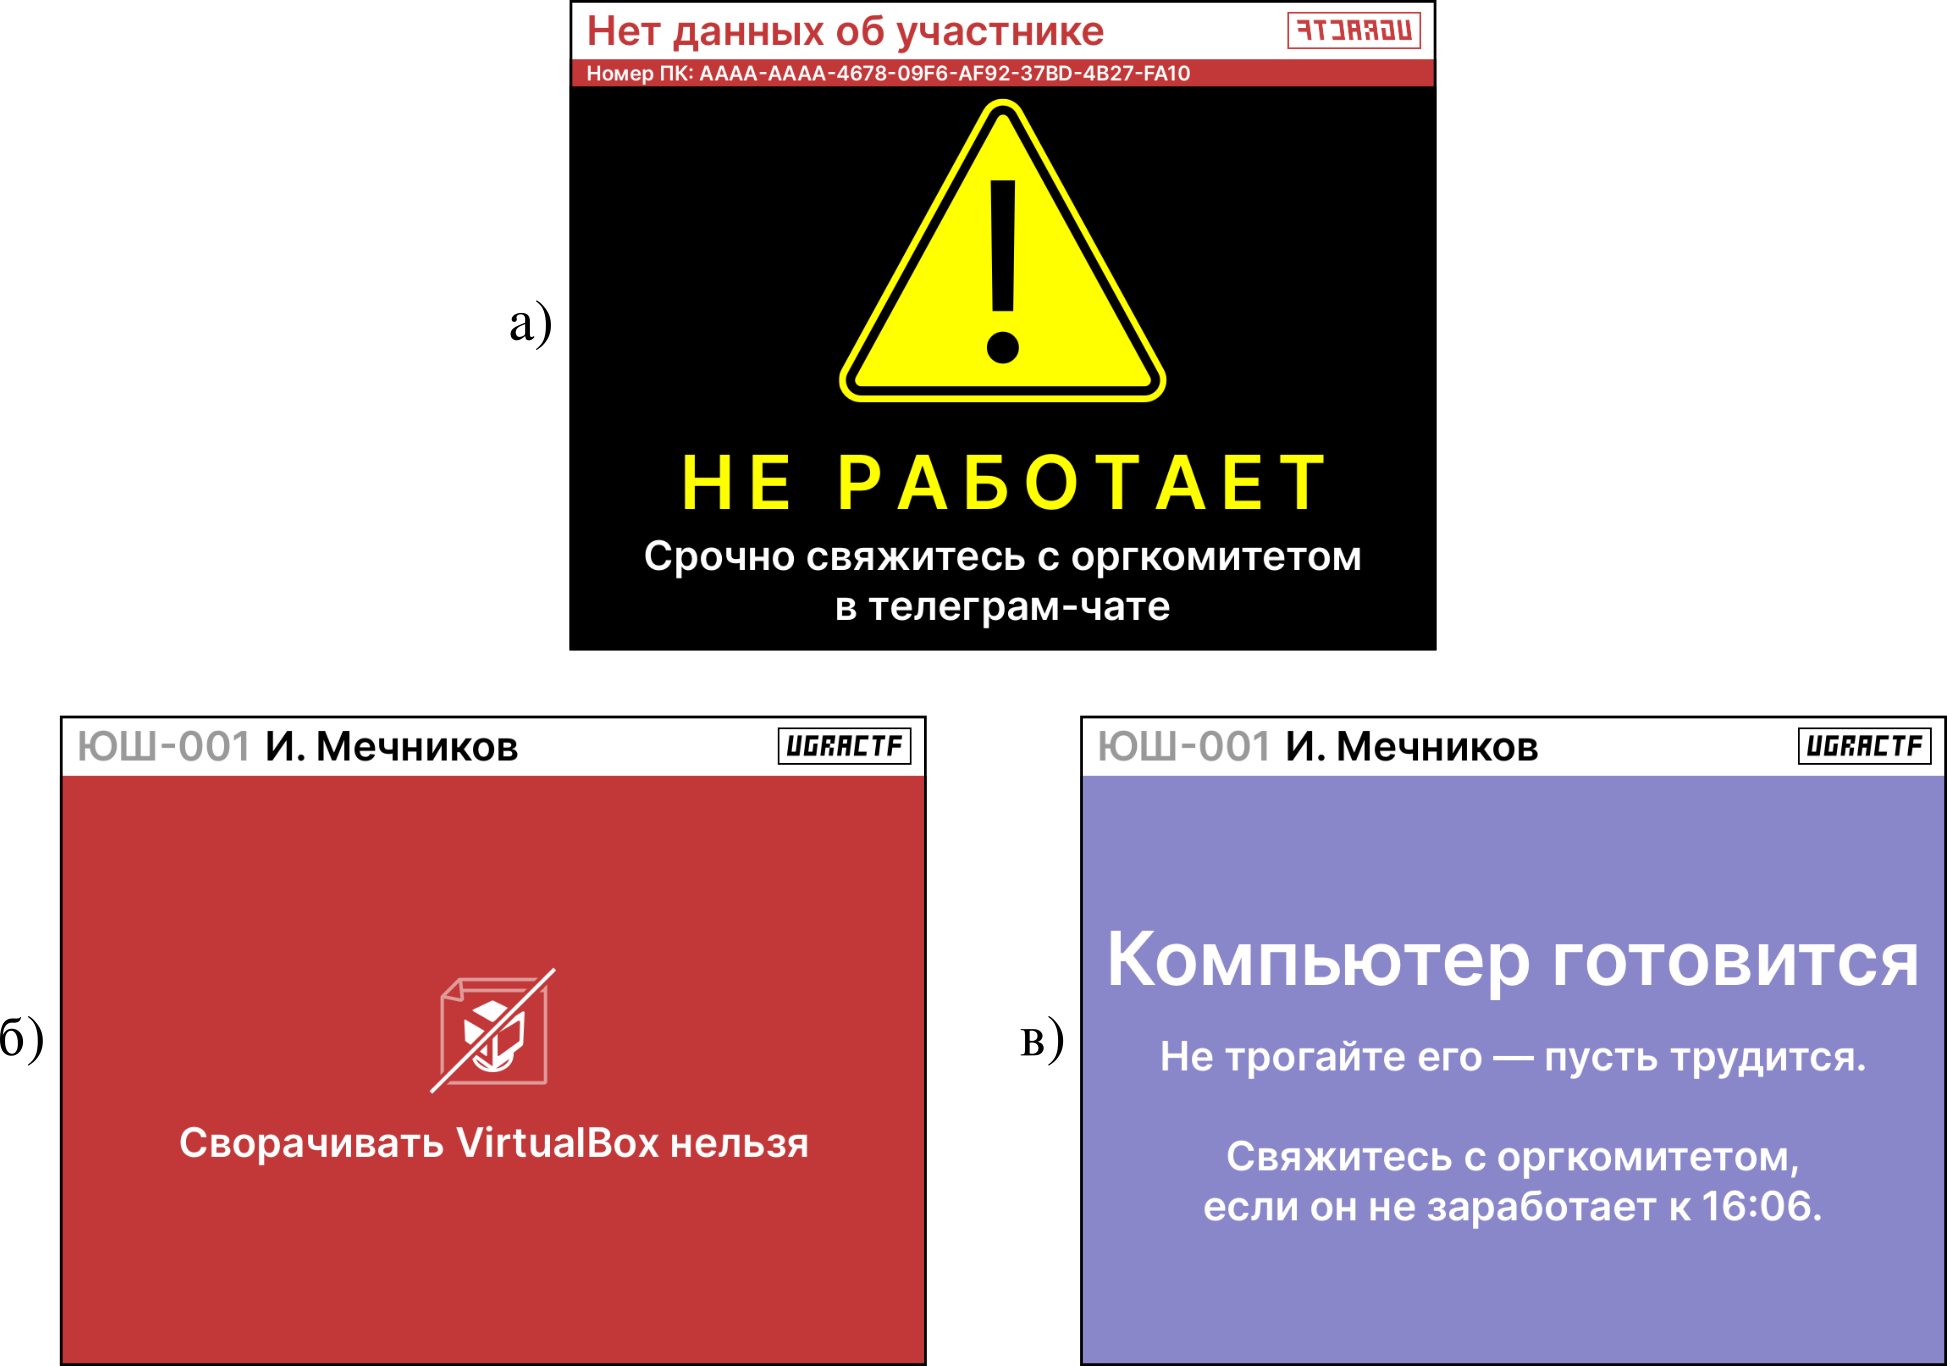
\includegraphics[width=1\textwidth]{inc/img/walls}
  \caption{Три вида индикации состояния системы: а) произошёл сбой; б) штатный режим работы; в) инициализация системы.}
  \label{fig:walls}
\end{figure}

Изображение может содержать произвольный текст~--- например, инструкцию для участника или наблюдателя в случае сбоя, а также диагностическую информацию. Чтобы упростить процесс рассадки участников за рабочие места, изображение также содержит фамилию и инициал участника и его шифр, набранные крупным текстом.

Красный фон изображения выбран неслучайно~--- по правилам олимпиады сворачивать ВМ с гостевой ОС нельзя, и в случае, если это произошло, благодаря яркости цвета, наблюдателю на площадке будет проще заметить данное нарушение.




\section{Модуль среды Kyzylborda}

Для разработки данного модуля применены язык программирования Python и база данных PostgreSQL. Выбор пал на эти технологии по причине того, что каждый разработчик оргкомитета хорошо знаком с ними, к тому же, основная ИС оргкомитета, <<Юрт>>, также написана и использованием этого же технологического стека.

Kyzylborda рассчитана за запуск в ОС NixOS и использует возможности, предоставляемые пакетным менеджером Nix для автоматической изолированной публикации ресурсов при игровых задачах.


\subsection{Модель данных}

Основная сущность в Kyzylborda~--- \texttt{users}. Она содержит в себе сведения для аутентификации участника, его идентификатор и прочие атрибуты.

\begin{figure}[h!]
  \centering
  \includegraphics[width=1\textwidth]{inc/dia/kyzyl.eps}
  \caption{Схема моделей и их отношений в базе данных Kyzylborda}
  \label{fig:kyzyl}
\end{figure}

Все остальные сущности привязаны к \texttt{users} (рисунок \ref{fig:kyzyl}).

Эти сущности связаны с непосредственными функциями, которые должна выполнять борда:
\begin{itemize}
\item \texttt{submitted\_flags} соответствует посылкам участников;
\item \texttt{generated\_tasks}~--- сгенерированным бордой вариантам игровых задач;
\item \texttt{generated\_flags}~--- флагам для этих \texttt{generated\_tasks};
\item \texttt{granted\_hints}~--- подсказкам (не используются в рамках текущего набора правил);
\end{itemize}



\subsection{Пользователь}

Пользователь обладает уникальным идентификатором, благодаря которому можно привязывать к нему другие сущности. Это необходимо для того, чтобы генерировать задачи по вариантам и определять авторов посылок для их оценки, составления рейтинга и~--- после испытания~--- предоставления итоговой отчётности.

Пользователь может быть организатором. Организатор видит в веб-интерфейсе дополнительные поля, содержащие диагностическую информацию, а также может сбрасывать кэш сгенерированных вариантов игровых задач. Посылки организатора проверяются, однако в рейтинге он не учитывается~--- это даёт возможность тестировать задачи прямо во время игры, не мешая участникам.

Пользователь также может быть дисквалифицирован. В этом случае он исключается из рейтинга, а в турнирной таблице возле его строки появляется соответствующая отметка.

Сущность пользователя определяет механизм аутентификации и авторизации, с помощью которого участник может воспользоваться веб-интерфейсом. Это может быть как авторизация по токену, которые загружаются в борду из ИС <<Юрт>>, так и более универсальная авторизация по паре логин-пароль на случай проведения CTF-соревнований, не относящихся к циклу Ugra CTF.

Наконец, пользователю можно присвоить одну или несколько меток~--- текстовых строк, с помощью которых можно как угодно делить участников на группы: например, по площадкам или виду зачёта (в отборочном этапе существует неофициальный зачёт для людей, которые не учатся в школе).

\subsection{Игровые задачи}

Игровые задачи борда принимает в виде директорий особой структуры. Рассмотрим её на конкретном примере~--- динамической задачи.

Эта задача~--- пример того, как можно использовать пакетный менеджер Nix, чтобы создавать нужное программное окружение. В качестве примера задача динамически запускает тривиальное веб-приложение на языке Python, использующее стороннюю зависимость~--- сервер Redis, а также создаёт во вложениях текстовый файл, содержащий косвенный идентификатор участника.

Она также генерирует динамические флаги.

Данные задачи хранятся внутри директории \texttt{tasks}. Структура директории нашей задачи, которая называется \texttt{nix-example}, видна на рисунке \ref{fig:tree}. В первую очередь задача определяется конфигурационным файлом вида \texttt{<название задачи>.yaml}. Он приведён ниже.

\begin{figure}[hb!]
  \centering
  \begin{verbatim}
                      nix-example
                      |-- app
                      |   |-- isolated_run_daemon.sh
                      |   |-- redis.conf
                      |   |-- run_daemon.sh
                      |   \-- server.py
                      |-- generator.py
                      |-- nix-example.yaml
                      \-- run_generator.sh
  \end{verbatim}
  \caption{Демонстрация страницы сгенерированной по варианту пользователя динамической игровой задачи: её страница и вложение}
  \label{fig:tree}
\end{figure}

\begin{lstlisting}[caption={Конфигурационный файл задачи \texttt{nix-example}}]
category:  lol   # категория задачи
points:    100   # стоимость в очках
author:    you   # имя или ник автора
title:     Nix-generated Task   # полное название для интерфейса
description: <p>So it goes.     # описание (HTML)

generator: ./run_generator.sh   # путь к генератору флагов

# описание фонового процесса - сервера веб-приложения
daemon:
    exec: ./run_daemon.sh   # путь к скрипту, запускающему сервер
    cwd: app                # рабочая директория сервера
    socket: app.sock        # серверу нужен выделенный сокет...
    socket_type: http       #   для обмена по протоколу HTTP
\end{lstlisting}

В конфигурационном файле перечислены все сведения, необходимые для того, чтобы сгенерировать флаги, описание и вложения задачи, а также запустить фоновый процесс. Остальные данные в директории задачи~--- непосредственно, программа-генератор и код веб-приложения.

Генератор~--- программа, принимающая на вход косвенный идентификатор пользователя и путь до директории для вложений. Она может создавать и записывать файлы в эту директорию. Генератор всегда возвращает JSON-объект со следующими полями:

\begin{itemize}
\item \texttt{flags}: уникальные флаги для этого варианта задачи;
\item \texttt{substitutions}: данные для подстановки в переменные, которые можно использовать в текстовом описании задачи;
\item \texttt{urls}:  ссылки на сопутствующие ресурсы (в нашем случае~--- на веб-сервер).
\end{itemize}

Код генератора этой задачи тривиален: он создаёт во вложениях файл, записывает в него полученный от борды косвенный идентификатор участника и формирует JSON-объект согласно описанной выше спецификации.

Скрипт, запускающий сервер~--- это исполняемый файл, приведённый ниже.

\begin{lstlisting}[caption={Скрипт, запускающий сервер}]
#!/usr/bin/env nix-shell
#!nix-shell -i bash -p python3 -p python3Packages.flask -p python3Packages.redis -p python3Packages.gunicorn -p redis

statedir="$1"
task_name="$2"

export BWRAP_PROPAGATE_MOUNTS="/bin /usr/bin /nix/store"
exec kyzylborda-isolate \
  --unshare-net \
  --bind "$1" "/state" \
  --bind "$TMPDIR" "/tmp" \
  --ro-bind "$PWD" "$PWD" \
  --chdir "$PWD" \
  -- ./isolated_run_daemon.sh
\end{lstlisting}

Он выполняется не командной оболочкой ОС, а утилитой \texttt{nix-shell}, что следует из первой строки. Вторая строка сообщает утилите, что мы хотим получить чистое программное окружение, содержащее пакеты: \texttt{python3}, \texttt{flask}, \texttt{redis}, \texttt{gunicorn}, которые необходимы для запуска веб-приложения. Наконец, скрипт использует программу Bubblewrap \cite{Bubblewrap}, с помощью которой создаётся изолированный контекст для процесса веб-сервера: он отделён от сетевых интерфейсов ОС и её файловой системы, за исключением рабочей директории, в которой содержатся его ресурсы и директории для временных файлов.

\begin{figure}[h!]
  \centering
  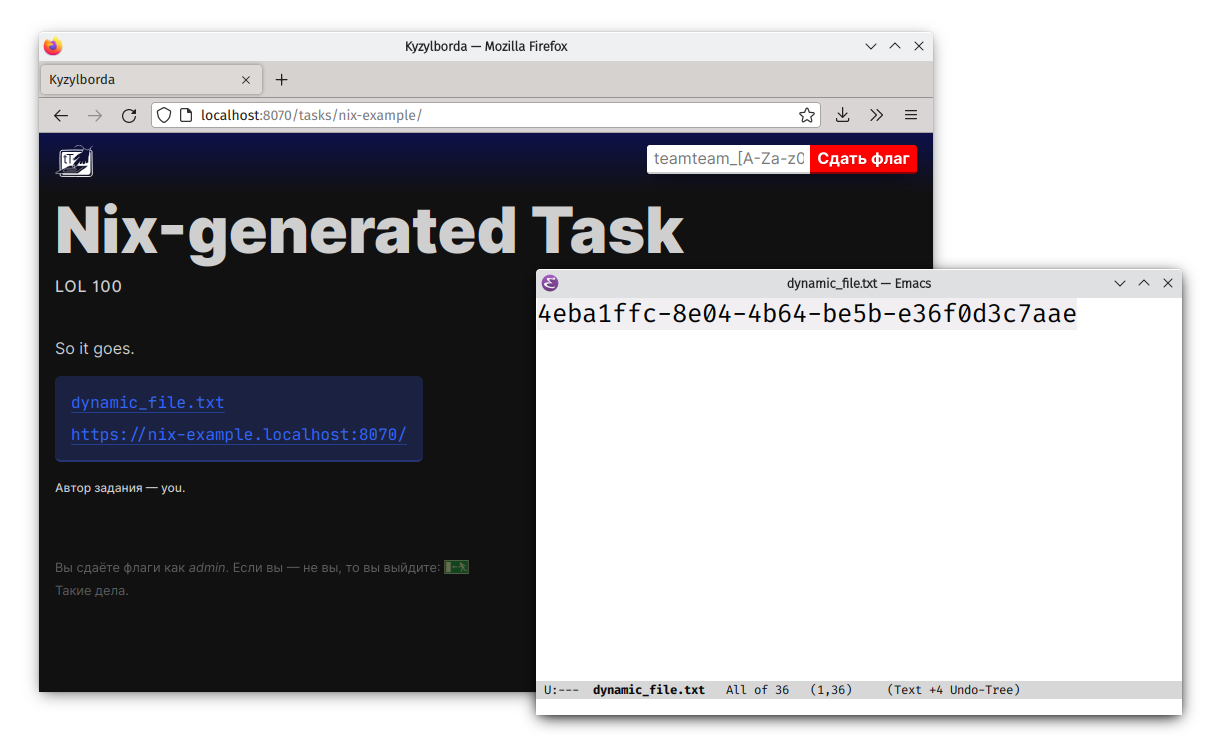
\includegraphics[width=0.92\textwidth]{inc/img/nix}
  \caption{Демонстрация страницы сгенерированной по варианту пользователя динамической игровой задачи: её страница и вложение}
  \label{fig:nix}
\end{figure}

Кроме запуска скрипта борда также автоматически обеспечивает корректную конфигурацию самого сервера~--- начинает принимать HTTP-трафик по адресу: \texttt{nix-example.<домен соревнований>} и перенаправлять его процессу веб-сервера, обеспечивая его доступность во внешней сети.

После размещения задачи в нужной директории и запуска борды, можно воспользоваться веб-интерфейсом, чтобы проверить, что задача, во-первых, начала отображаться в интерфейсе, во-вторых, при переходе на её страницу действительно генерируется вариант для текущего пользователя, соответствующий формальному описанию задачи (рисунок \ref{fig:nix}).

За запуск и остановку процессов отвечает системная служба \texttt{supervisord} \cite{supervisord}. В ней реализованы безопасные и надёжные механизмы управления задачами, и она предоставляет возможность управления посредством программного интерфейса. Благодаря использованию этой технологии и введению корректных абстракций в коде модуля Kyzylboard, процессы, связанные с задачами, могут использовать в целях изоляции и обеспечения воспроизводимой программной среды не только Nix, но и технологии контейнеризации, например, Docker \cite{Docker}.


\subsection{Интерфейс}

Для веб-интерфейса используется библиотеку Flask \cite{Flask}. Она позволяет создать веб-сервер и определить его поведение: создать т.н. маршруты \textit(англ. routes)~--- правила, которые определяют, как обрабатывать тот или иной HTTP-запрос в зависимости от его типа или содержимого.

Интерфейс рассчитан на использование в браузере. Код страниц для браузера формируется из шаблонов, логика которых изолирована от основной логики модуля Kyzylborda. Это согласуется с принципами модульной архитектуры, описанными в Главе 2.

С помощью веб-интерфейса участники получают доступ к турнирной таблице, описаниям задач и сдают свои посылки. Все посылки принимаются веб-сервером и записываются в базу данных как сущности типа \texttt{submitted\_flags}.



\section{Выводы}

В данной главе была рассмотрена подробная модель автоматизированной системы, предоставляющей среду для проведения дистанционных испытаний в области защиты информации, отражающая структуру её программных компонент.

В результате проведённой работе были разработаны два основных модуля системы и изучены особенности, связанные с их реализацией.


\backmatter %% Здесь заканчивается нумерованная часть документа и начинаются ссылки и

%\Conclusion % заключение к отчёту

В результате проделанной работы стало ясно, что ничего не ясно...

%%% Local Variables: 
%%% mode: latex
%%% TeX-master: "rpz"
%%% End: 
%% заключение


% % Список литературы при помощи BibTeX
% Юзать так:
%
% pdflatex rpz
% bibtex rpz
% pdflatex rpz

% \bibliographystyle{gost780u}
% \bibliography{rpz}

\setlength\bibhang{0pt}

\defbibenvironment{bibliography}
{\list
{\printfield[labelnumberwidth]{labelnumber}}
{\setlength{\labelwidth}{\labelnumberwidth}%
\setlength{\leftmargin}{0cm}%
\setlength{\labelsep}{\biblabelsep}%
%\addtolength{\leftmargin}{\labelsep}%
\setlength{\itemsep}{\bibitemsep}%
\setlength{\parsep}{\bibparsep}}%
\renewcommand*{\makelabel}[1]{\hss##1}}
{\endlist}
{\item}

\printbibliography[heading=bibintoc,title={Список литературы}]
%%% Local Variables:
%%% mode: latex
%%% TeX-master: "rpz"
%%% End:



%\appendix   % Тут идут приложения

%\chapter{Исходные коды модуля SchoolOS}
\label{cha:appendix1}

\lstinputlisting[caption={flake.nix}]{inc/src/schoolos/flake.nix}

\lstinputlisting[caption={client/default.nix}]{inc/src/schoolos/client/default.nix}
\lstinputlisting[caption={client/module.nix}]{inc/src/schoolos/client/module.nix}
\lstinputlisting[caption={client/platform.nix}]{inc/src/schoolos/client/platform.nix}
\lstinputlisting[caption={client/usb.nix}]{inc/src/schoolos/client/usb.nix}

\lstinputlisting[caption={server/default.nix}]{inc/src/schoolos/server/default.nix}
\lstinputlisting[caption={server/handle-proxy.sh}]{inc/src/schoolos/server/handle-proxy.sh}
\lstinputlisting[caption={server/handle-proctor.sh}]{inc/src/schoolos/server/handle-proctor.sh}
\lstinputlisting[caption={server/ssh-to-client.sh}]{inc/src/schoolos/server/ssh-to-client.sh}
\lstinputlisting[caption={server/remote-customize.sh}]{inc/src/schoolos/server/remote-customize.sh}

\lstinputlisting[caption={customize-image.sh}]{inc/src/schoolos/customize-image.sh}
\lstinputlisting[caption={prepare-provision.sh}]{inc/src/schoolos/prepare-provision.sh}

%%% Local Variables:
%%% mode: latex
%%% TeX-master: "rpz"
%%% End:


%\chapter{Еще картинки}
\label{cha:appendix2}
\blindtext

\begin{figure}
\centering
\caption{Еще одна картинка, ничем не лучше предыдущей. Но надо же как-то заполнить место.}
\end{figure}

%%% Local Variables: 
%%% mode: latex
%%% TeX-master: "rpz"
%%% End: 


\end{document}

%%% Local Variables:
%%% mode: latex
%%% TeX-master: t
%%% End:
